\chapter{Related Work}
\label{cha:related-work}

% Miner history -> Goldstrike -> Heterogenity -> Heterogenity + bitcoin mining

Because of bitcoins popularity and the competitiveness involved in mining it, there exists
many different accelerators to improve the performance and energy efficiency of mining systems.
During the currency's history, hardware for bitcoin mining has evolved from regular, general-purpose
CPUs to highly specialized ASIC chips.

Likewise, heterogeneous systems have evolved as an answer to dark silicon problems inherent in
modern processor chips. Different solutions utilizing different aspects of Taylor's proposed
solutions from section \ref{sec:taylor} are harnessed in new hardware.

\section{History of Bitcoin Mining}

The bitcoin blockchain was started on January 3rd, 2009. At this point, all mining was done
using CPU mining. The official bitcoin network client supports mining and was used for this
purpose. The fastest CPU miner, a high-end, overclocked Core i7 990x eventually reached 33~MH/s
using SIMD extensions in order to improve performance. \cite{bitcoin-history}

\subsection{GPU Mining}
The shift to GPU mining started in July 2010, when the first OpenCL miner was written and
used in a private mining setup. In September that year, the first open source GPU miner
was released after the author was paid 10~000 bitcoins, worth about \$600 USD at the time,
by Jeff Garzik, one of the core bitcoin developers. An open source OpenCL-based miner was
released shortly after \cite{bitcoin-history}.

OpenCL miners typically computes the double SHA256 hash using a fully unrolled implementation
of the compression loop. Multiple calculations are run simultaneously exploiting the parallelism
offered by GPUs. Many miners tweaked parameters of their hardware, such as the voltage and
clock frequencies of both the video RAM and the GPU core in order to get higher throughput
and thus reduce the cost of running each GPU, in order to obtain greater profits \cite{bespoke-silicon}.

\subsection{FPGA Mining}

FPGA miners appeared in June 2011, providing better power efficiency as compared to GPUs \cite{bespoke-silicon}.
Early designs were mostly based on the Spartan 6 FPGAs from Xilinx, and could provide a
performance of between 200~MH/s and 220~MH/s per chip, about the same as contemporary GPUs \cite{bitcoin-hardware-cmp}
but consuming as little as a fifth of the power used by their GPU counterparts \cite{bespoke-silicon}.

% Note: Taylor managed to get the release year of the GPUs he compares performance to wrong,
% choosing GPUs from 2012 to compare to FPGAs from 2011.

FPGAs provided great advantages to the speed of bitwise functions, which are important for
the SHA256 algorithm. Popular open-source designs were created so that they could be used
by different kinds of FPGAs. They consisted of a SHA-256 module which could be configured
with a specific unroll factor, that is, they had a configurable depth pipeline, each
consisting of the neccessary hardware for computing a specific number of rounds of the
SHA256 compression function. Completely unrolling the algorithm created a pipeline of
64 stages, with a throughput of 1 hash per cycle, while it was also possible to specify
lesser unroll factors which resulted in fewer pipeline stages and reduced throughput, taking
several cycles to perform a hash but saving registers and logic resources in the FPGAs.
The pipelines were duplicated to improve performance.

Power consumption became much higher than typical for FPGAs, with the pipelined design
giving extremely high activity factor for LUTs. Pre-made boards could not provice enough
power nor heat dissipation to sustained usage, and hackers thus developed custom
boards that focused on providing enough power and cooling with minimal unused resources,
such as RAM and I/O components. \cite{bespoke-silicon}

\subsection{ASIC Miners}

Neither GPUs nor GPUs can compare to ASICs, specialized chips that started to appear on the network
in the beginning of 2013 \cite{first-asic-miner}. It was the need for more high-performance and power
efficient bitcoin miners caused implementors of bitcoin miners to turn to ASIC solutions.

One of the first ASIC designs were Butterfly Labs' ASIC miners. Having experience developing
FPGA based mining solutions, the company created an ASIC chip with 16 double SHA256 modules,
the equivalent of 16 FPGA-based miners using a 65~nm process. The end-product ended up being
delayed when the chips ended up consuming more power than expected and had to be underclocked
in order to be able to cool the chips properly.

ASICMINER was another of the earliest designs, including only one SHA256 hash unit on a chip,
replicating a single FPGA-based design at a much higher frequency, with better power efficiency
and a cheaper price. \cite{bespoke-silicon}

\subsubsection{The Goldstrike 1}
Another ASIC design is the Goldstrike 1 architecture, noteworthy because its architecture is
described in an article in IEEE Micro. Because of the competitive nature of bitcoin mining,
it is not common for designers of ASIC solutions to reveal too many details about the architecture
of their chips and few scientifi papers exist on the topic.

The Golstrike is an ASIC-based bitcoin mining solution capable of reaching 2~TH/s. To reach the performance
requirements, a bitcoin mining core was created that was able to perform at 125 GH/s. Four of
these were combined in one package, with four of these packages then combined on a circuit board
to produce the target performance.

The Goldstrike cores consist of an architecture with 120 hash engines running in parallel.
A hash engine searches through all possible values of the 32-bit nonce field in the bitcoin header
(see section \ref{sec:bitcoin-mining}) in order to find a valid hash.

The hash engines uses a pipelined double-SHA256 implementation, with each round of the hash calculation
unrolled into a pipeline.

Tinished ASIC chips, each with four bitcoin mining cores, was measured to provide 504~GH/s while using
500~W of power. This gives a power efficiency of about 1~GH/J.

Interestingly, the architecture provided challenges when it comes to powering and cooling the chips.
Because the architecture uses all available computing power for bitcoin mining all the time while
the chips are in use, no parts of the chips can be turned off to save power. \cite{goldstrike}

% Fun fact, GH/Ws = GH/J

\subsection{Scaling of bitcoin hardware}
Due to the dark silicon problem, future chips will require that parts of it must be powered down or deactivated,
in order to satisfy a given power budget\cite{dark-silicon2}. As mentioned, bitcoin mining may be close to
the worst case for dark silicon optimizations, far beyond multicore CPUs or GPUs. Due to bitcoin mining's high procesing requirements, the logic needed to run the algorithm cannot be turned off without losing
performance.

BLF ran into this problem with their 65~nm chip, and had to scale back the performance to reduce power consumtion
and manage to cool the chip properly. While bitcoin mining began as a ``race to ASIC'', energy costs now determines
which ASICs are the most profitable and thus energy efficiency is a problem that must be addressed. \cite{bespoke-silicon}

\section{Heterogeneous Processors}

Heterogenenous architectures offers various possibilities for improved performance and energy efficiency;
this could be in the systems ability to adapt to various applications or even external conditions such as
power or temperature conditions \cite{heterogeneous-ee, heterogeneous-perf, heterogeneous-arch}.

%Kumar \textit{et al} \cite{heterogeneous-ee, heterogeneous-perf, heterogeneous-arch} explores the diverse possibilities offered by heterogeneous architectures. 
%They prediction that core diversity will be of higher value than uniformity, and will offer much greater ability to adapt to the demands of the applications.
%They argue that the objective function can change over time, such as power conditions, application switches, or changes of demands within the application\cite{heterogeneous-ee}. 

\subsection{Energy Efficiency}
\label{subsec:rw_ee} 
Kumar \textit{et al}\cite{heterogeneous-ee} ran a simulation where they combined four generations from the Alpha family: EV4 (Alpha 21064), EV5 (Alpha 21164), EV6 (Alpha 21264) and a single-threaded version of EV8 (Alpha 21464), and made a heterogenous multi processor.
Only one application would run at the time, on one core, while the others were powered down.
The architecture, with the chosen cores and their relative sizes to one another can be seen in figure
\ref{fig:Kumar1}.

\begin{figure}[htb]
    \centering
    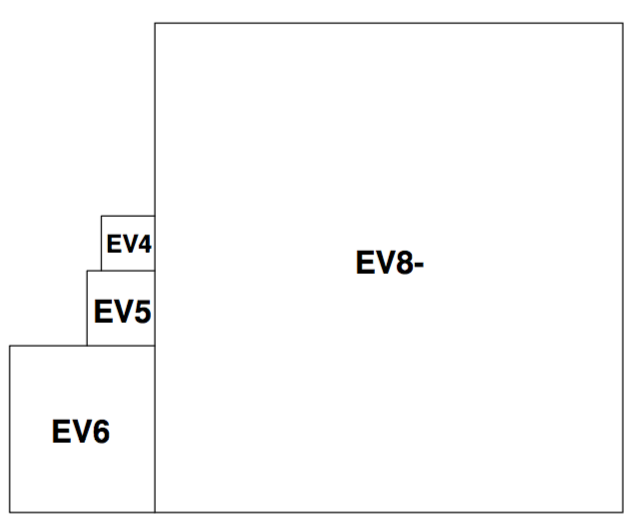
\includegraphics[width=0.5\textwidth]{Figures/Heterogeneous/Kumar1}
    \caption{Cores used in \cite{heterogeneous-ee}, and their relative sizes.}
    \label{fig:Kumar1}
\end{figure}


14 benchmarks from SPEC2000 were used in this experiment, simulated using SMTSIM, and both energy and energy-delay were measured.

For the simulation, it was assumed that the system knew the needs of every application, and selected core statically. 
Results showed average energy savings of 32\%, and average performance loss at only 2.6\%, relative to using the EV8 core.
Kumar \textit{et al} also used this experiment to show that dynamic core switching outperforms the best static core selection.
Simple heuristics would sample the cores at regular intervals, and execute core switch based on the results.
The heuristics achieved up to 93\% of the energy-delay gains compared to the best static selection. 

\subsection{Performance}
\label{subsec:rw_perf}
In another experiment, Kumar \textit{et al}\cite{heterogeneous-perf} proved that heterogeneity can be exploited to gain increased performance, for multithreaded workload.
They point out that heterogeneous architectures are advantagous for two reasons.

Firstly, they offer efficient adaptation to application diversity, as applications differs in their resource needs.
Some are compute intensitive and make good use of an out-of-order pipeline with high issue-width, while others may be memory-bound, and will underutulize advanced cores.
They may perform almost as well on an in-order core with low issue-width\cite{heterogeneous-perf}.

Secondly, heterogeneous architectures offers more efficient use of the die area for a given thread-level parallelism.
A complex core can be replaced by multiple smaller and simpler cores. 
Since the process or thread-level paralellism varies within most systems, a mix of cores that offers some large cores for high single-thread performce, and some small cores with high throughput per die area, is a potentially attractive area. \cite{heterogeneous-perf}

In contrast to the previous work described in \ref{subsec:rw_ee} by Kumar \textit{et al}, this experiment assigned multiple threads for multiple cores, and best global assignment was considered above best assignment for a selected application.
EV5 and EV6 from the Alpha family were chosen for this project, with one EV6 nearly equal to five EV5 in size.
With the total chip area anvailable for the architecture assumed to be 100 mm$^2$, the space could consist of maximum 4 EV6 cores, or 20 EV5 cores.
Three EV6 cores and five EV5 were chosen for this experiment, with expectation that it would perform well over a wide range of available thread-level parallelism. 
A small number from SPEC2000 benchmarks were chosen, with the focus on evaluating varying number of threads.
SMTSIM and Simpoint were used for the simulation.

%\todo{Mind-blowing, consider removal}Evaluation metric was weighted speedup, which in this context is the arithmetic sum of the individual IPCs of the threads constituting a workload divided by their IPC on a baseline configuration when running alone.
%In addition to performance gain, application response time within varying queue lengths is tested as well, to give insight on how well heterogeneous processors handles large queues, compared to best homogeneous systems.

Best static scheduling ensures that threads that are least affected by the difference between the EV5 and the EV6, are assigned to the EV5 processors, when all EV6 processors are occupied.
When the number of threads passes 4, the measured weighted speedup increases on the heterogeneous system, compared to a homogeneous CMP with 4 EV6.
When the number of threads passes 13, a CMP with 20 EV5 performs better, though this can be changed with a different combination of EV5 and EV6 cores.
This is shown in figure \ref{fig:Kumar2}.

%\todo{Following 2 sentences are nearly ripoff from \cite{heterogeneous-perf}, consider making quote or what?}
Compared to 4 EV6 cores, the heterogeneous processor performed up to 37\% better with an average 26\% improvement over the configuration considering 1-20 threads. 
Compared to 20 EV5 cores, the performance was up to 2.3 times better, and averaged 23\% better over that same range. \cite{heterogeneous-perf}
Using dynamic heuristics for core assignment further increased the performance.

\begin{figure}[htb]
    \centering
    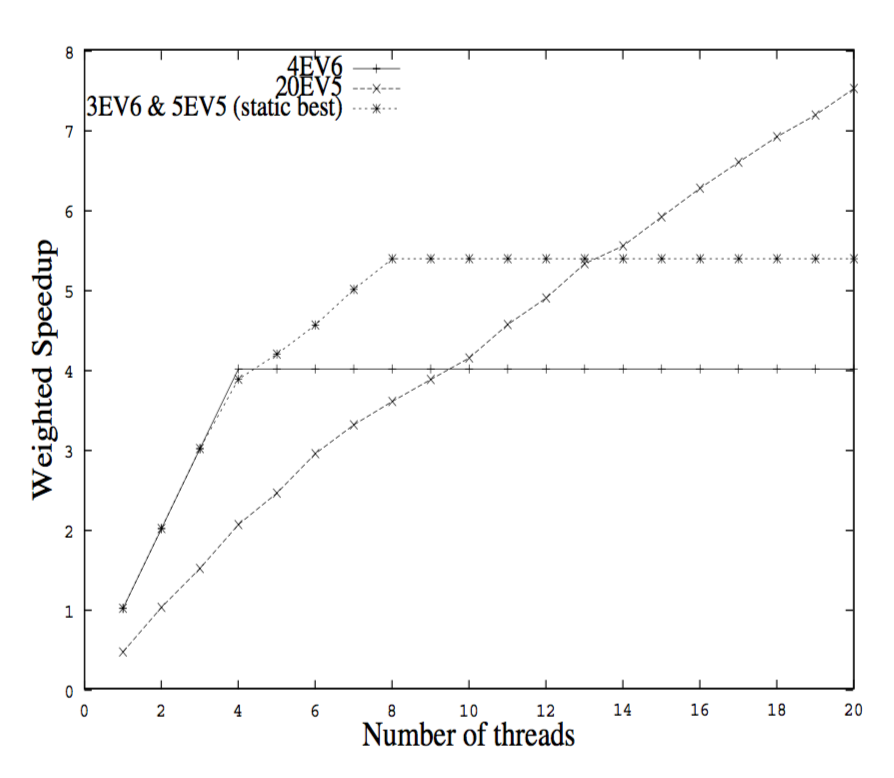
\includegraphics[width=0.5\textwidth]{Figures/Heterogeneous/Kumar2}
    \caption{Benefits from heterogeneity - static scheduling for inter-thread diversity, as seen in \cite{heterogeneous-perf}.}
    \label{fig:Kumar2}
\end{figure}

In addition to testing the performance gain, Kumar \textit{et al} also tested the the response time within queue lenght as well.
This was to give insight on how well heterogeneous processors handles large job queues, compared to best homogeneous systems.
%For testing response time in an open system, and how various que length affects it, jobs with an average distrubition of 200 million cycles were generated randomly and executed.
For this test, jobs with an average distrubition of 200 million cycles were generated randomly and executed.
Then different mean job arrival rates with exponential distribution were simulated.
It was revealed a great difference between saturation for a homogenous system with 4 EV6, and the heterogeneous processor.
For the former, the unbounded response time is seen as the arrival rate approached its maximum throughput around 2 jobs per 100 million cycles.
From there, the run queue became infinate.
The heterogeneous system remained stable well beyond that point.
The degredation was also more graceful under heavier loads than for homogeneous processors.
This can be seen in figure \ref{fig:Kumar3}.

\begin{figure}[htb]
    \centering
    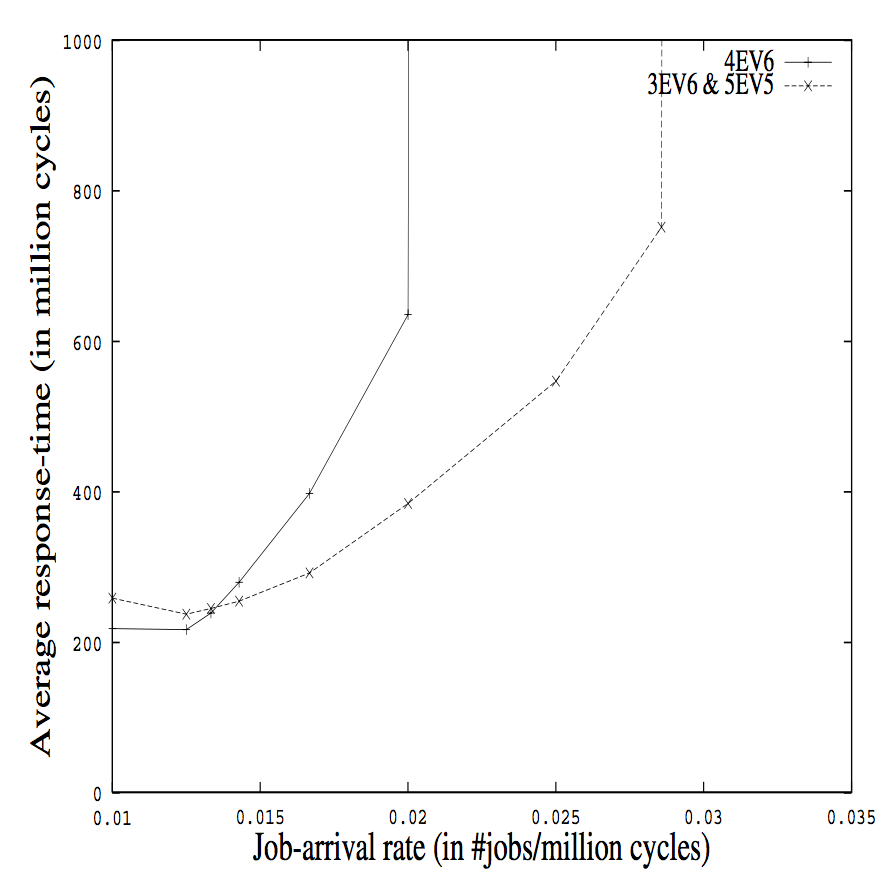
\includegraphics[width=0.5\textwidth]{Figures/Heterogeneous/Kumar3}
    \caption{Limiting response-time for various loads, as seen in \cite{heterogeneous-perf}.}
    \label{fig:Kumar3}
\end{figure}

\subsection{Optimal architecture}
\todo{Subchapter needs double check against source papers}
\label{subsec:rw_arch}
Kumar \textit{et al}\cite{heterogeneous-arch} has taken a closer look at what is good heterogeneous design.
They argue that while the previous experiments gave increased energy efficiency and performace, a heterogeneous system should be designed from scratch, instead of using pre-existing core designs.
While they surpassed homogeneous designs, pre-existing cores failed to reach the full potential of heterogeneousy for three reasons: They present low flexibility in choices, the core choices remain monotonic, and best heterogeneous design are composed of specialized core architectures\cite{heterogeneous-arch}.
But also, if pre-existing cores are not used, additional costs in design, verification and testing must be evaluated, to see if the benefits are worth the cost.

They made three significant contributions in this experiment. 
First, benefits of heterogeneity in power and area efficient architectures is re-evaluated, with new benefits and higher gains shown.
Secondly, methodologies for for arriving at good heterogeneous designs are demonstrated.
Thirdly, a number of key principles critical to effective design of future chip multiprocessors are identified.

Several conclusions were derived:
%\todo{Itemize or cut down at this point}
The most efficient heterogeneous multiprocessors were not constructed from cores that make good general-purpose uniprocessor cores, or cores that would appear in a good homogeneous multicure architecture.
Each core was individually tuned for a class of applications with common characteristics.
The results are usually non-monotonic processors.
And performance advantages of heterogeneous multiprocessors, including non-monotonic also holds for completely homogeneous workloads.
In those cases, the diversity across different workloads are exploited.

%\todo{Just a headnote. Remove when agreed or fixed}\textbf{Simplification assumptions dropped}

%A number of 480 unique cores could be made from the various parameters set for this experiment.
%\todo{Makes absolutely sense at all. Cut down or delete, but some way explain what the parameters were.}These were the issue width, I-cache size, D-cache size, L2 Cache size, Memory Channel, number of FP-IntMul-ALU units, IntQ-fpQ and IntFp PhysReg-ROB (OOO), ITLB-DTLB and LD/St Queue.
%\todo{Mention the "best fit" problem from monotonic cores?}
%\textbf{Insert mentioned todo-content or remove. And find suitable place}

A fixed number of four cores were used for this experiment.
In addition to testing the various core builds, the combinations were tested against varying area and power constraints, with their performance compared to the best homogeneous multiprocessors.
Static mapping were mainly used for this experiment, but few tests with dynamic mapping showed further increase in performance, since a thread could be moved around to most suitable core at any phase of its execution. 

%\todo{Strongly considering deleting (commenting out) the following paragraph. Too much unnecessary details.}The workloads come from seven benchmarks from the SPEC suite, classified int o processor bound or bandwidth bound.
%The chosen benchmarks are carefully selected, and represents the entire SPEC suite.
%In additional, three other benchmarks from other suites are chosen as well.
%Every multiprocessor is evaluated on two classes of workloads, called \textit{all different} and \textit{all same}.
%\todo{Warning: Direct rip-off. Consider "quote"-form}The former consist of all possible 4-threaded combinations that can be constructed such that each of the 4 threads running at a different time.
%The latter consists of all combinations that can be constructed so that all the 4 threads running at a time are the same.

%\todo{Direct copy, rewrite the paragraph}We use weighted speedup [21] for our evaluations. In this paper, weighted speedup measures the arithmetic sum of each running thread’s IPC, divided by its IPC on the simplest core considered in this study when running alone. The IPC is derived by running a thread for a fixed amount of time. We believe that this metric guards against multiprocessor design points that produce artificial speedups by simply favoring high-IPC threads.
%For completeness reasons, we also performed all our evaluations for total IPC as well and found that while the absolute results were different, there was no significant difference in trends or analysis.

It turned out that the more constricted the anvailable power or chip area, the more gain custom heterogeniety provided, as homogeneous multiprocessors could only perform any task at maximum if the power budget was generous.
But as designs become more aggressive, one will want to place more cores on the die, and power budgets per core is likely to tighten more severly.
Heterogeneous designs dampen the effects of constrained power budgets \cite{heterogeneous-arch}.

Any best heterogeneous design for the different tested power and area constraint were very different from best homogeneous design, underlining the need to design heterogeneous processors from a clean slate, rather than modifying an existing core design.
Monotonous designs (for instance, different generations of cores from same family) does not exploit heterogeneity equally well.
For instance, the benchmark \textit{mcf} from \cite{heterogeneous-ee} were mapped on EV6 or single-threaded EV8-, in spite of having low ILP.
The reason was the larger caches of these cores, causing the advances capabilities of these larger cores to be underutulized.

Heterogeneous multicore processors designed from clean slate gives better performance.

%\subsection{Uncore}
%\todo{Client worklod description has been cut out. Reconsider if it should be included}
%\label{subsec:rw_uncore}
%Gupta \textit{et al}\cite{heterogeneous-uncore} ran experiments with a heterogeneous multiprocessor, with the goal of measuring the impact of "uncore" power on the energy efficiency of heterogeneous multicore processors.
%In this experiment, they focused on the use of client devices, where energy is a premium resource and the workload profiles are diverse.
%The uncore is a collection of components of a processor, not in the core, but essential for core performance.
%Some of these components are the last level cache (LLC), integrated memory controllers (IMC), on-chip interconnect (OCI), power control logic (PWR), etc.
%With growing cache size and integration of various SoC components on the CPU die, the uncore is becoming an increasingly imporant contributor \cite{heterogeneous-uncore}.

%If a core has varying levels of sleep states, where the "deeper the sleep", the less power used, then uncore will be as active as the most active core.
%If three cores are idle (or on low activity), and one core is on highest activity, then the uncore will be on the highest activity.
%If for a task, the choice is between a big fast core, or a more power efficient small core, and the small core is chosen, the ucore will stay active for longer time, impacting the possible energy saving.
%This can be seen illustrated in figure \ref{fig:Uncore1}.

%\begin{figure}[htb]
%    \centering
%    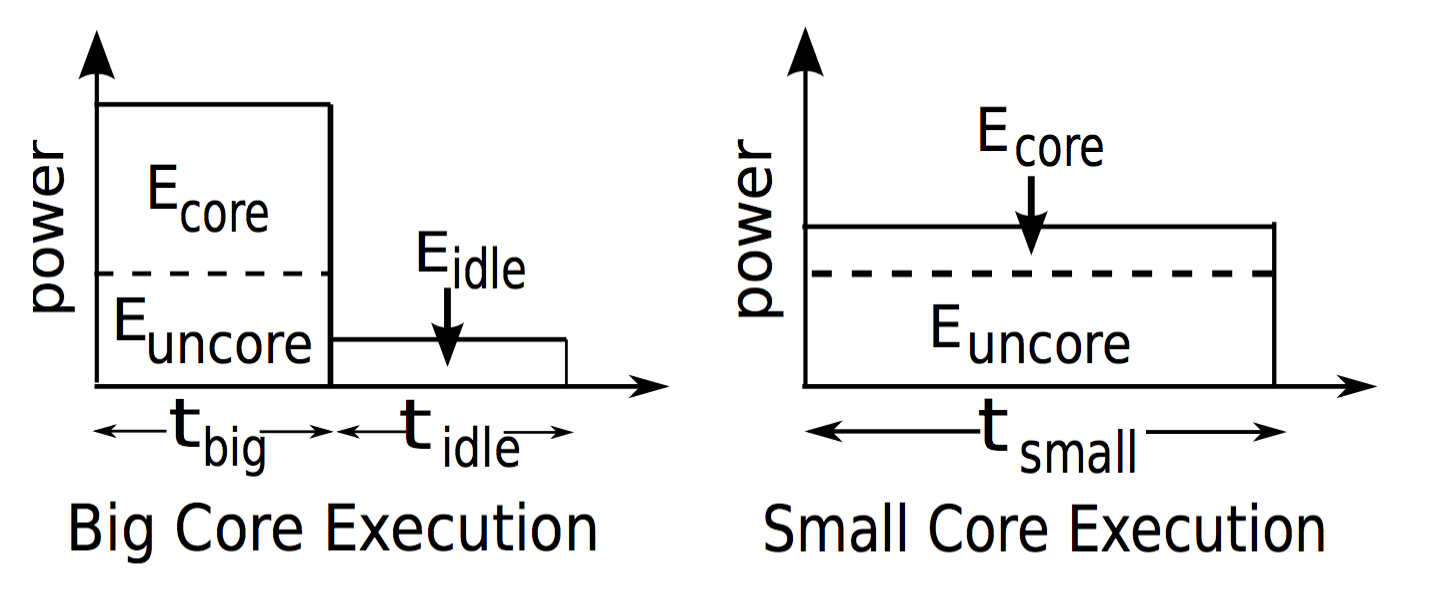
\includegraphics[width=1.0\textwidth]{Figures/Heterogeneous/Uncore1}
%    \caption{Effect of uncore power on the energy efficiency of heterogeneous cores, as seen in \cite{heterogeneous-uncore}.}
%    \label{fig:Uncore1}
%\end{figure}


%\todo{WARNING}\textbf{Skipped client workload description}

%The analysis considered two uncore conficurations: fixed and scalable.
%The first one used the same uncore subsystem for both big and small cores.
%The second modeled an uncore where certain components were turned off or powered down when moving to small cores.
%Examples are fewer memory channels, controllers, or smaller caches used.  

%\begin{figure}[htb]
%    \centering
%    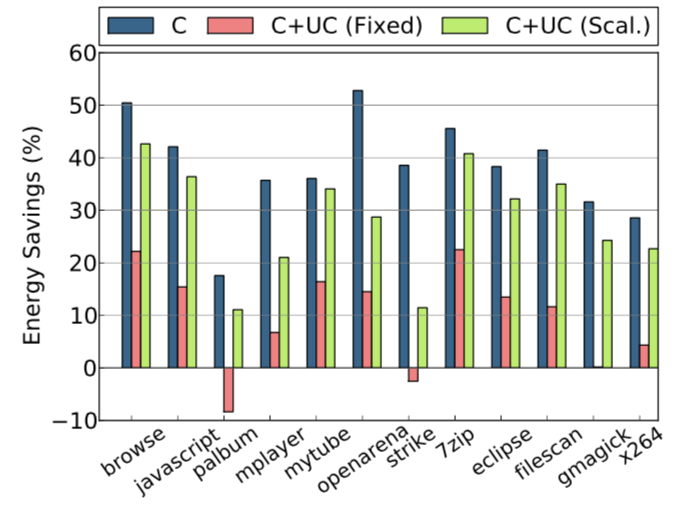
\includegraphics[width=1.0\textwidth]{Figures/Heterogeneous/Uncore2}
%    \caption{Energy savings of using small cores, with core-only savings (C), and with SoC-wide savings (C+UC), with a fixed uncore, and with a scalable uncore, as seen in \cite{heterogeneous-uncore}.}
%    \label{fig:Uncore2}
%\end{figure}

%Figure \ref{fig:Uncore2} shows the energy saved when going from big to small core, with both fixed and scaled uncores.
%It is clear that without scaling of the uncores, energy saving is reduced, even wasted in some cases.
%Figure \ref{fig:Uncore3} shows the relative contribution of core and uncore energy consumption for all the applications during big core execution, on a fixed uncore configuration.

%Clearly it is important to take uncore power into account for scheduling operations, and design of scalable uncore design is motivated, to obtain better gains from heterogeneous multicores. 

%\begin{figure}[htb]
%    \centering
%    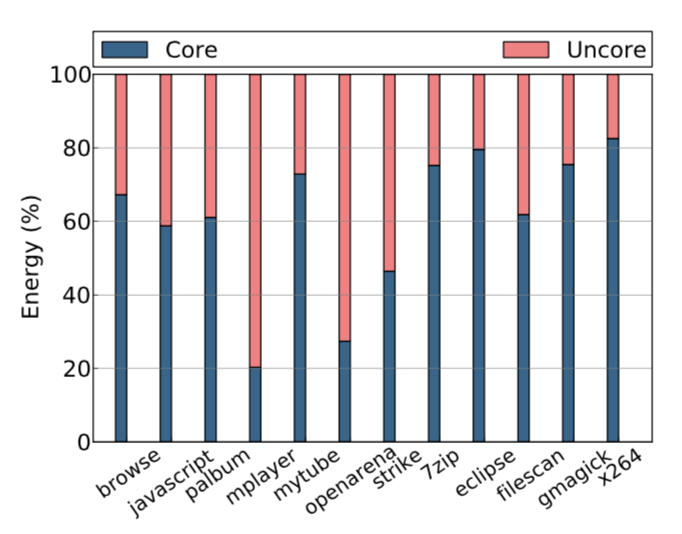
\includegraphics[width=1.0\textwidth]{Figures/Heterogeneous/Uncore3}
%    \caption{Core and uncore energy contricution for big cores and fixed uncores, as seen in \cite{heterogeneous-uncore}.}
%    \label{fig:Uncore3}
%\end{figure}

\section{Heterogenity and Bitcoin Mining}

Because of the need for all available computing power to solve hashes, heterogeneous architectures
may not seem the best solution for 

Heterogeneous systems may be configured to include bitcoin mining as an application. This can be
done by either making a complete, separate bitcoin mining core in a heterogeneous computer
or by incorporating an accelerator into an existing core or as a peripheral in such a system.

The Zedboard is a platform using a Zynq-7020 system-on-chip from Xilinx, which consists of
two Cortex-A9 processors, various peripherals and an FPGA area. This platform was evaluated
as a possible bitcoin mining platform, by using a separate bitcoin mining
accelerator. The accelerator included hardware for accelerating both the double SHA-256 calculation
and for comparing the result with the target value. At 50 MHz they obtained a performance of about
0.8~MH/s. \cite{xcell-bitcoin,standridge-master}

